\documentclass{article}

\usepackage{indentfirst}
\usepackage{setspace}
\doublespacing

% ================================================================================= 
% Package for showing source code
% ================================================================================= 

\usepackage{listings}
\usepackage{color}

\definecolor{dkgreen}{rgb}{0,0.6,0}
\definecolor{gray}{rgb}{0.5,0.5,0.5}
\definecolor{mauve}{rgb}{0.58,0,0.82}

\lstset{frame=tb,
language=C,
aboveskip=.5mm,
belowskip=.5mm,
showstringspaces=false,
columns=flexible,
basicstyle={\scriptsize\ttfamily},
numbers=none,
numberstyle=\tiny\color{gray},
keywordstyle=\color{blue},
commentstyle=\color{dkgreen},
stringstyle=\color{mauve},
breaklines=false,
breakatwhitespace=true,
tabsize=3
}

% ================================================================================= 
% Package for flowcharts/diagrams
% ================================================================================= 

\usepackage{tikz}
\usetikzlibrary{shapes.geometric, arrows}

\tikzstyle{startstop} = [rectangle, rounded corners, minimum width=3cm, minimum height=1cm,text centered, draw=black, fill=red!30]
\tikzstyle{io}        = [rectangle, minimum width=3cm, minimum height=1cm,text centered, draw=black, fill=blue!30]
\tikzstyle{process}   = [diamond, minimum width=2cm, minimum height=0cm, text centered, draw=black, fill=orange!30]
\tikzstyle{arrow}     = [thick,->,>=stealth]

% ==================================================
% Paper
% ==================================================

\title{Fully Generalized Compilation}
\date{01-26-2017}
\author{Lucas Saldyt}

\begin{document}

\maketitle
\pagenumbering{gobble}
\newpage
\pagenumbering{arabic}

% ==================================================
\section{Abstract}
% ==================================================
Glossa is an investigation into the feasibility of a multi-language source-to-source compiler with dynamic grammars. 
Assuming that two languages are \textit{isomorphic}, one language can be converted to another if given an adequate description of each language's grammar.
At an abstract level, this conversion is entirely practical. Given source code in one language, a description of its grammar \textbf{A} , and a description of an output language's grammar \textbf{B}, can \textbf{A} be converted to \textbf{B} such that the output in \textbf{B} is indistinguishable from a program originally written in \textbf{B}?
Once this is achieved, the grammar description for \textbf{A} can be modified, and the program will still output code in the \textbf{B} language that satisfies the above constraint.

% ==================================================
\section{Introduction}
% ==================================================

A multi-language source to source compiler is potentially a tool for programming language researchers, providing a \textit{dynamic framework} for easily modifying syntax of input and output languages. 
Glossa also uses this concept to re-implement existing source-to-source compilation tools, such as \textbf{Cython} or \textbf{2to3}.

% ==================================================
\section{Methods}
% ==================================================

\subsection{Compilation}
Traditionally, a compiler takes a single high-level programming language, and converts it into machine instructions.
\begin{enumerate}
\item Code is lexed (seperated into tokens and tagged as keywords, punctuators, literals, etc...)
\item Tokens are parsed to build an abstract syntax tree (symbolic code representation)
\item The AST is optimized (i.e. unreachable code is removed, some loops are unrolled)
\item Machine instructions are generated from AST.
\end{enumerate}
While some compilers and interpreters have dynamic ways to modify the syntax of a language, this functionality seems to be unneeded for most compilers.

Glossa differs only slightly from the steps above. Lexing and parsing work as above, but the rules for lexing and parsing respectively are read in at run-time. 
In the current state of the software, optimizations don't occur, but could easily be modeled as transformations to the abstract syntax tree.
Instead of generating machine instructions, Glossa generates code in another programming language. 
Instructions for doing this are also read in at run-time.
Because of its dynamic nature, it is very simple to have Glossa support multiple programming languages both for input and output.

\subsection{Abstracting Language Definitions}

To parse an input language, Glossa needs a description of the languages grammar, which is provided through a \textit{grammar file}.
Optional descriptions of AST transformations are provided through \textit{transformer files}.

To generate an output language from an AST, Glossa needs a set of \textit{constructor files}.

\subsection{Grammar Files}

Glossa's parse operation can be modeled as a function with the signature:

parse :: Tokens -> AST

Where the body of the parse function looks like:

\lstset{language=Python}
\begin{lstlisting}
while not tokens.empty():
    identify_remaining(tokens)
\end{lstlisting}

Glossa will attempt to identify remaining tokens with any of the high-level statement types provided.
These statement types can use other grammar constructs as well

A single grammar files defines a potential identification of tokens, producing a tagged dictionary of symbols if the tokens are identified successfully:

The simplest non-trivial grammar file is likely the assignment statement:

\verbatim
assignment: `@lval identifier **` `@op '='` `@rval boolexpression | expression`
\end{verbatim}

In plain english this reads:
"Parse an identifier, and save it to the symbol dictionary as `lval`, then parse an equals operator, and save it to `op`, lastly, parse a boolean expression or normal expression and save it to `rval`"

In general, a grammar element is defined like the following:

\verbatim
name: `first_element` `second_element`
\end{verbatim}

Where first\_element and second\_element are parsers of the form:

\verbatim
an optional "@name" tag, which saves the result of the parser to the symbol dictionary under "name"
Either:
- A subtype parser (i.e `'='`),
- A subtype-type parser (i.e. `identifier self`)
- A type parser (i.e. `identifier **`)
- A link to another grammar element (i.e. `value`)

So, the following are all examples of valid parsers:
`@val value`          // Link to value type, saved as "val"
`identifier self`     // Identifier "self", discarded
`@name identifier **` // Any identifier saved as "name"

However, these parsers can be prefixed with the following keywords to change their meaning:

!           : discard the parse result of this parser
anyOf a b   : parse either a or b, keeping the result of the first successful parser. This has syntactic sugar of the form (a | b)
*/many      : parse the parser several times until it fails
many1       : parse the parser several times, requiring it to parse successfully at least once
optional    : make a parser optional
inOrder a b : run several parsers in order
sep a b     : parse bs seperated by as (i.e. sep , value) 

Some examples of more sophisticated parsers

`@statement import_from | main | ... ` 
`@val identifier ** | string | literal ** | 'None' | 'True' | 'False'`
`@val vector | functioncall | elementaccess | memberaccess | basevalue | parenexpr`
`@args optional sep ',' expression`

\end{verbatim}


\subsection{AST Transformations}

Reasoning for and description of AST-transformations

\subsection{Constructors}

Description of Constructor implementation

\newpage

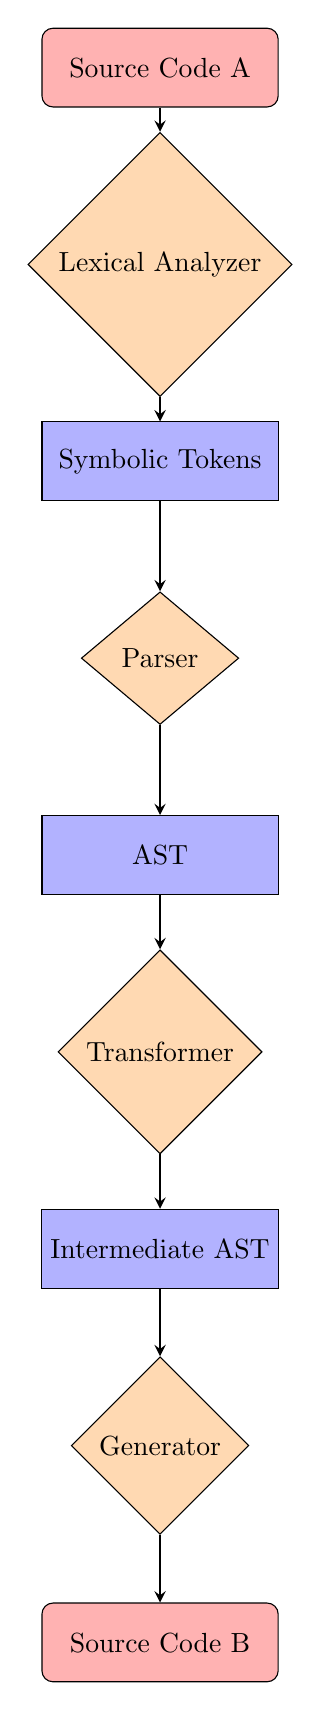
\begin{tikzpicture}[node distance=2.5cm]

    \node (sourcea) [startstop]                 {Source Code A};
    \node (lexer)   [process, below of=sourcea] {Lexical Analyzer};
    \node (tokens)  [io, below of=lexer]        {Symbolic Tokens};
    \node (parser)  [process, below of=tokens]  {Parser};
    \node (asta)    [io, below of=parser]       {AST};
    \node (trans)   [process, below of=asta]    {Transformer};
    \node (astb)    [io, below of=trans]        {Intermediate AST};
    \node (gen)     [process, below of=astb]    {Generator};
    \node (stop)    [startstop, below of=gen]   {Source Code B};

    \draw [arrow] (sourcea) -- (lexer);
    \draw [arrow] (lexer) -- (tokens);
    \draw [arrow] (tokens) -- (parser);
    \draw [arrow] (parser) -- (asta);
    \draw [arrow] (asta) -- (trans);
    \draw [arrow] (trans) -- (astb);
    \draw [arrow] (astb) -- (gen);
    \draw [arrow] (gen) -- (stop);

\end{tikzpicture}


% ==================================================
\section{Applications}
% ==================================================

\subsection{Re-implementation of Cython and 2to3}
Description of implementing these two pieces of software with glossa

\subsection{Cython}
\subsection{2to3}

\subsection{Comparisons and Benchmarks}

\subsection{Simple code porting}
Reference work on 2to3, talk about FORTRAN and similar conversions

\subsection{Language Creation}
Description of implementing new programming languages using glossa

\subsection{Language Design and Modification}
\subsection{Glossa as a pre-processor}

% ==================================================
\section{Results}
% ==================================================

\subsection{Results Overview}

2to3 comparison

Cython comparison

GHC comparison

\subsection{Quicksort Cython Comparison}

\newpage
\subsection{Original Python Code}

\lstset{language=Python}
\begin{lstlisting}
def sort(array):
    less    = []
    equal   = []
    greater = []

    if len(array) <= 1:
        return array
    else:
        pivot = array[0]
        for x in array:
            if x < pivot:
                less.append(x)
            if x == pivot:
                equal.append(x)
            if x > pivot:
                greater.append(x)
        return sort(less) + equal + sort(greater)

def main():
    l = sort([3, 2, 12, 9, 4, 68, 17, 1, 2, 3, 4, 5, 6, 12, 9  , 8, 7, 6,5, 4, 743])

if __name__ == "__main__":
    main()
\end{lstlisting}

\lstset{language=C}

\newpage
\subsection{Generated C++ Code (Glossa)}

\begin{lstlisting}
#include "../std/std.hpp"
template <typename T_array>
auto sort (T_array array)
{
    auto less = std::vector<Object>({});
    auto equal = std::vector<Object>({});
    auto greater = std::vector<Object>({});
    if (len(array) <= 1)
    {
        return array;
    }
    else
    {
        auto pivot = array[0];
        for (auto x : array)
        {
            if (x < pivot)
            {
                less.push_back(x);
            }
            if (x == pivot)
            {
                equal.push_back(x);
            }
            if (x > pivot)
            {
                greater.push_back(x);
            }
        };
        return sort(less) + equal + sort(greater);
    };
}
\end{lstlisting}

\newpage
\subsection{Generated C Code (Cython)}

Generated code for Cython is much more complex, as it integrates with the Python FFI

For example, this snippet declares an empty array

\begin{lstlisting}
  /* "main.py":6
 *     Sorts an array of comparable values
 *     """
 *     less    = []             # <<<<<<<<<<<<<<
 *     equal   = []
 *     greater = []
 */
  __pyx_t_1 = PyList_New(0); if (unlikely(!__pyx_t_1)) {__pyx_filename = __pyx_f[0]; __pyx_lineno = 6; __pyx_clineno = __LINE__; goto __pyx_L1_error;}
  __Pyx_GOTREF(__pyx_t_1);
  __pyx_v_less = ((PyObject*)__pyx_t_1);
  __pyx_t_1 = 0;
\end{lstlisting}

\newpage

% ==================================================
\section{Conclusion}
% ==================================================

\end{document}
